\section{General Design}
\label{sec:general_design}

This section is dedicated to the discussion of the general design of \snowman{}.

\subsection{Centralized or Distributed Setup?}
\label{sec:architecture_discussion}
We decided early on to design \snowman{} to be a distributed system. The main
considerations behind this choice were the bandwidth usage needed by the rule
updates, and the load on the central server.

\begin{figure}[h!]
	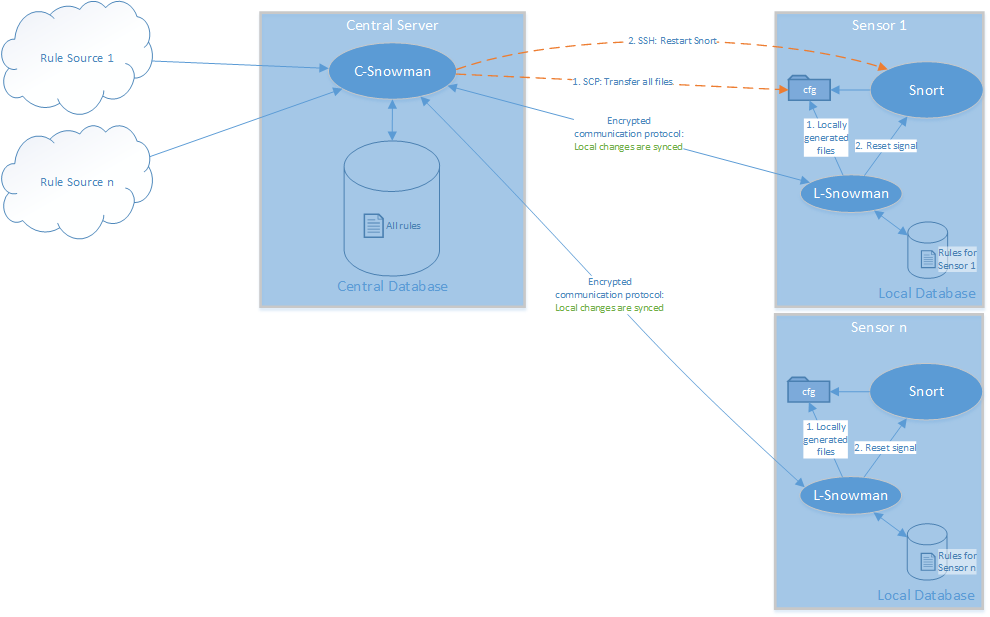
\includegraphics[width=200mm,angle=90]{./img/Architecture.png}
	\caption{General architecture}
	\label{fig:general_architecture}
\end{figure}

In Figure \ref{fig:general_architecture} we can see the difference between a
centralized and a distributed setup. The red dotted lines represent the
communication in a centralized setup, while the blue lines between the
server and the clients represent the communication in a distributed
setup. The latter is the principle used in \snowman{}.

\subsubsection{Bandwidth Requirements} 
The \snort{} sensors managed by \snowman{} might have varying
network infrastructure connecting them with the central server. In a worst case
scenario, the sensor might be located at a military base in the field, on the
other side of the planet, only connected to the central server via a satellite
connection with limited capabilities for transmitting data. As the rulesets applied to sensors
typically consist of tens of thousands of rules and the changes between two
versions of the sets typically only affect about a thousand of them, it seems
reasonable to only copy the changes when an update should be done. This is
achieved by using a distributed system.

\subsubsection{Central Server Load}
When a full update of all the sensors is requested, new rulesets would have to
be created and distributed to the sensors.

In a centralized environment, the central server would need to generate all
the new rulesets and send them to the sensor. The server
would not know beforehand which rules currently exist on the sensor, so a full list of rules
would need to be sent, even if there were no changes to any of the rules. Also,
if the sensor for some reason is unavailable, or connected through an unreliable
network connection, the central server would waste a lot of extra effort to
send the rules to the sensor, even if it is not neccesary as no rules have
changed.

In a distributed environment, we would be able to put some logic (a client) into
the machines hosting the sensors. This way, when an update is occurs, the
client can get a list of rules from the central server, and on its own accord
be responsible for collecting the new revision of the rules that have changed or
are missing. In this way, the central server would only need to transmit the
rules from its database if the rule is actually needed by the sensor.



